\documentclass{article}
\usepackage{report}

\makeatletter
\newcommand{\HEADER}[1]{\ALC@it\underline{\textsc{#1}}\begin{ALC@g}}
	\newcommand{\ENDHEADER}{\end{ALC@g}}
\makeatother
%opening
\date{2016年11月}
\title{货郎担问题实验报告}

\newcommand{\huo}{货郎担问题}

%\\heyihui@stu.xjtu.edu.cn
\begin{document}
\begin{CJK}{UTF8}{gkai}
%gkai gbsn
\begin{figure}
\centering
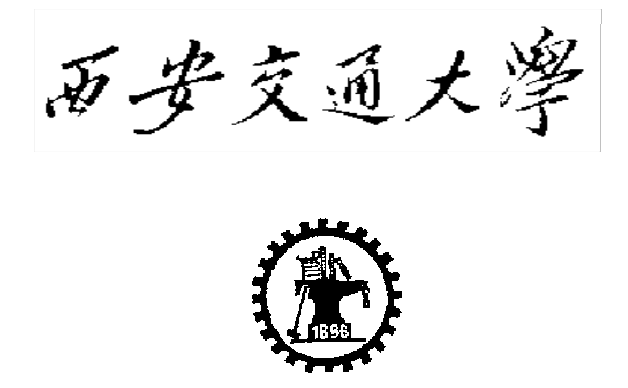
\includegraphics[width=0.6\linewidth]{xjtu}
\end{figure}
\maketitle
\clearpage

\section{实验内容}
探究货郎担问题,从某个城市出发,每个城市只允许访问一次,最后又回到原来的城市,寻找一条最短距离的路径。\cite{bao2010}
\section{实验目的}
货郎担问题TSP (Traveling Salesman Problem),又称旅行推销员或旅行商问题。由于问题本身的组合特性,其求解计算量随着城市的个数n增加而呈指数关系增长,穷举搜索法虽然能保证得到全局最优解,但面临着计算量组合爆炸的困难。

本实验探究了对于货郎担问题的不同解决方案。

\section{实验原理}
\begin{figure}
	\centering
	\includegraphics[width=.7\linewidth]{../TSP-paper/egtsp}
	\caption{}
	\label{fig:egtsp}
\end{figure}

正确得说,\huo 的距离定义是广义的,可以是图表示,连接表示。这样比较复杂。在本实验中仅仅考虑几何货郎担问题,根据三角形定义如下:
\begin{equation}
dist(A, C) < dist(A, B) + dist(B, C)
\end{equation}
这样的好处是,方便直观地显示出来,如图\ref{fig:att} 是美国城市的一个 \huo 最优解。


本实验采用学术界标准的.tsp 格式\cite{data1}来表示城市,文件第一行为城市的个数,剩下的行利用(坐标x,坐标y)的二元组来表示城市。下面给出一个例子:
\begin{lstlisting}
15
-0.0000000400893815        0.0000000358808126
-28.8732862244731230       -0.0000008724121069
-79.2915791686897506       21.4033307581457670
-14.6577381710829471       43.3895496964974043
-64.7472605264735108      -21.8981713360336698
-29.0584693142401171       43.2167287683090606
-72.0785319657452987       -0.1815834632498404
-36.0366489745023770       21.6135482886620949
-50.4808382862985496       -7.3744722432402208
-50.5859026832315024       21.5881966132975371
-0.1358203773809326       28.7292896751977480
-65.0865638413727368       36.0624693073746769
-21.4983260706612533       -7.3194159498090388
-57.5687244704708050       43.2505562436354225
-43.0700258454450875      -14.5548396888330487
\end{lstlisting}

\begin{figure}[!h]
	\centering
	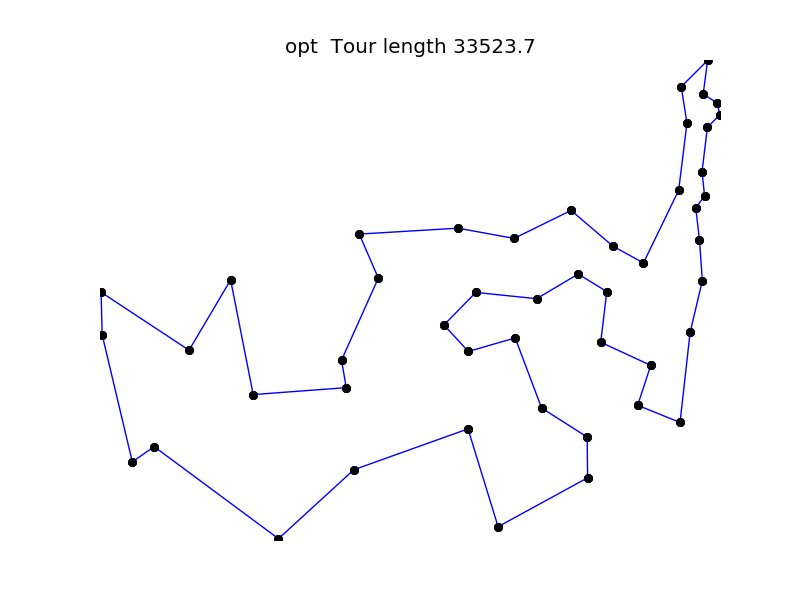
\includegraphics[width=.7\linewidth]{00000}
	\caption{最优路径}
	\label{fig:att}
\end{figure}

\section{程序代码}
在这里概述了主要的算法实现,具体代码请参见对应的程序文件。
\subsection{随机路径}
随机路径比较简单,仅仅是将顺序序列打乱,随机访问。
\begin{lstlisting}[language=python]
np.random.choice(n,n,replace=False)
\end{lstlisting}

\subsection{贪心算法}
类似于弗洛伊德算法,每加入一个城市后,考虑是否需要改变与新城市相连的节点。\cite{gutin2007greedy}
\lstinputlisting[language=python]{greedy.py}

\subsection{二优化算法}
随机选取路径出现重叠的两条路径,通过消解重叠的路径,降低总路程,克服了贪心算法的缺陷。\cite{croes1958method}
\lstinputlisting[language=python]{opt.py}

\subsection{退火算法}
模拟退火算法来源于固体退火原理,将固体加温至充分高,再让其徐徐冷却,加温时,固体内部粒子随温升变为无序状,内能增大,而徐徐冷却时粒子渐趋有序,在每个温度都达到平衡态,最后在常温时达到基态,内能减为最小。

有点类似二优化算法,不同之处在于,退火算法有一定随机性,有时候甚至会增加总路径(变异,取决与温度),容易逃离局部极小值。初始的温度应当足够高,才能保证系统找到足够好的解。\cite{grefenstette1985genetic}

\lstinputlisting[language=python]{sa.py}

\section{实验结果分析}
	在美国地图\huo 中,图\ref{fig:att}给出了最优解,图\ref{fig:rand}给出了随机产生的路径结果,图\ref{fig:greedy}给出了贪婪算法的结果\ref{fig:2opt},图\ref{fig:sa}给出了模拟退火算法的结果。
\begin{figure}[!h]
	\centering
	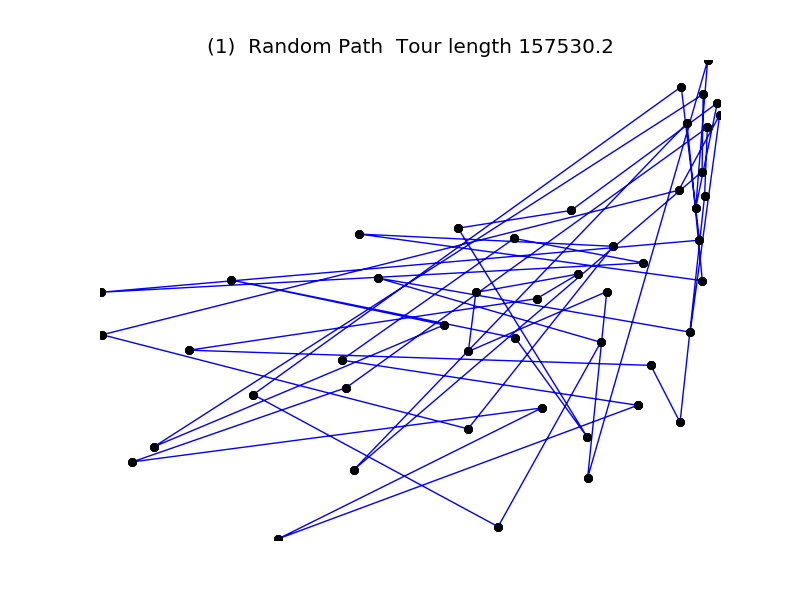
\includegraphics[width=.7\linewidth]{00074}
	\caption{随机路径}
	\label{fig:rand}
\end{figure}

\begin{figure}
	\centering
	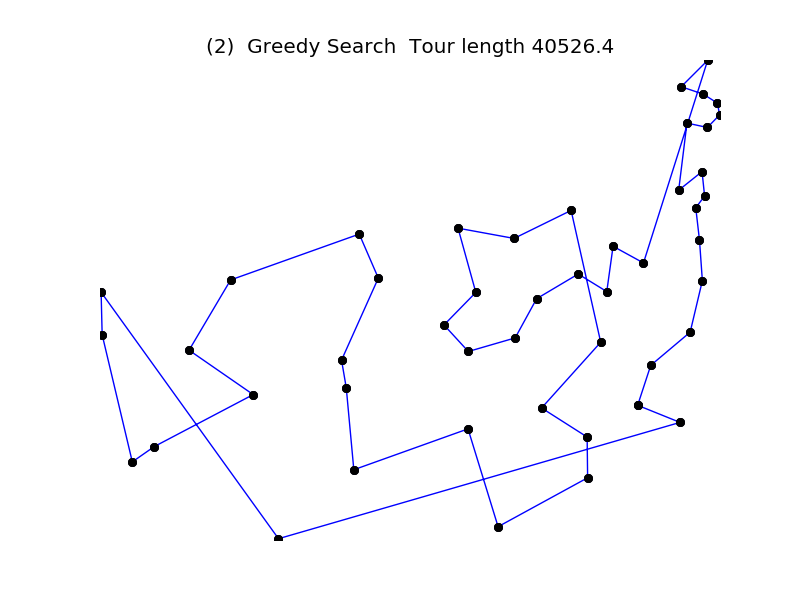
\includegraphics[width=.7\linewidth]{00226}
	\caption{贪心算法}
	\label{fig:greedy}
\end{figure}

\begin{figure}
	\centering
	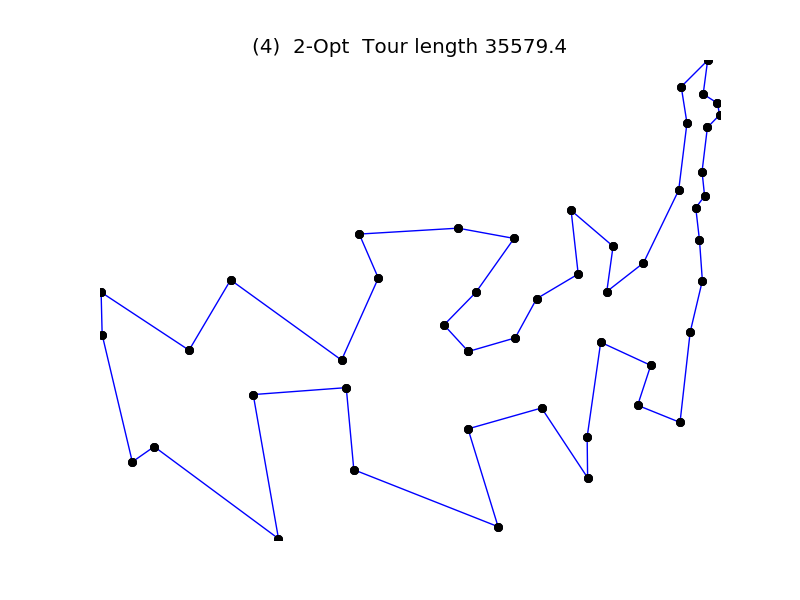
\includegraphics[width=.7\linewidth]{00322}
	\caption{二优化算法}
	\label{fig:2opt}
\end{figure}

\begin{figure}
	\centering
	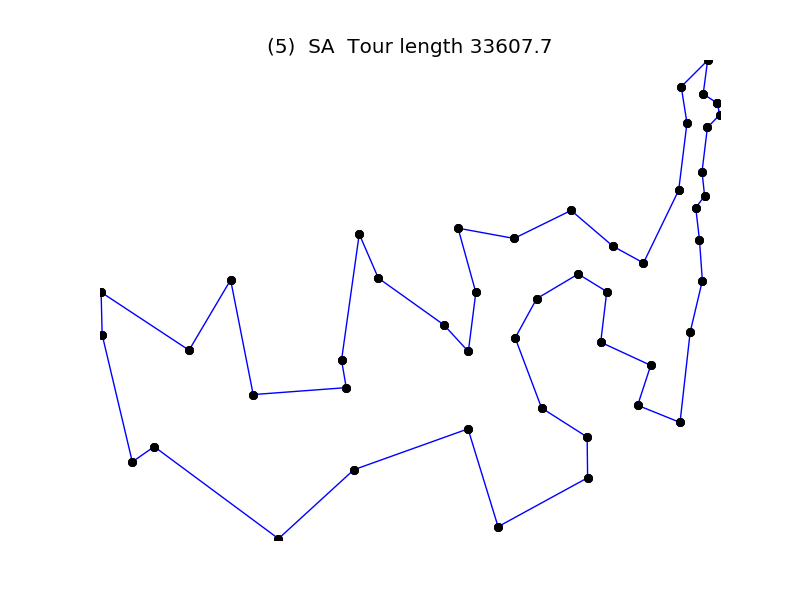
\includegraphics[width=.7\linewidth]{02132}
	\caption{退火算法}
	\label{fig:sa}
\end{figure}

如\ref{fig:path}所示,在小型数据集上,所有算法都差不多。然而在较大的数据集上,退火算法展示了较好的效果。

\begin{figure}[!h]
	\centering
	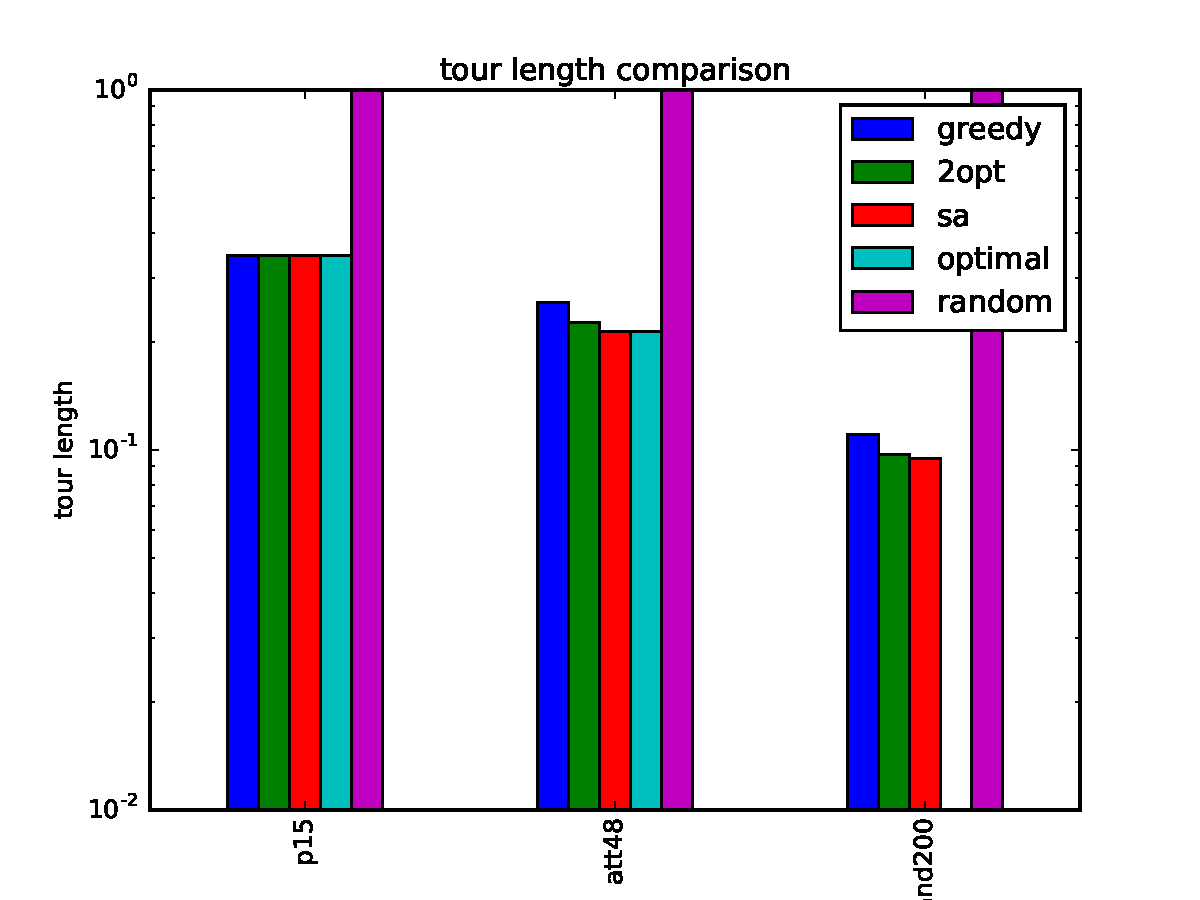
\includegraphics[width=.7\linewidth]{length}
	\caption{路径长度分析}
	\label{fig:path}
\end{figure}
如\ref{fig:time}所示,二优化算法的时间消耗随着数据集增大,呈指数爆炸形式,而退火算法和贪心算法表现出了较高的效率。
\begin{figure}[!h]
	\centering
	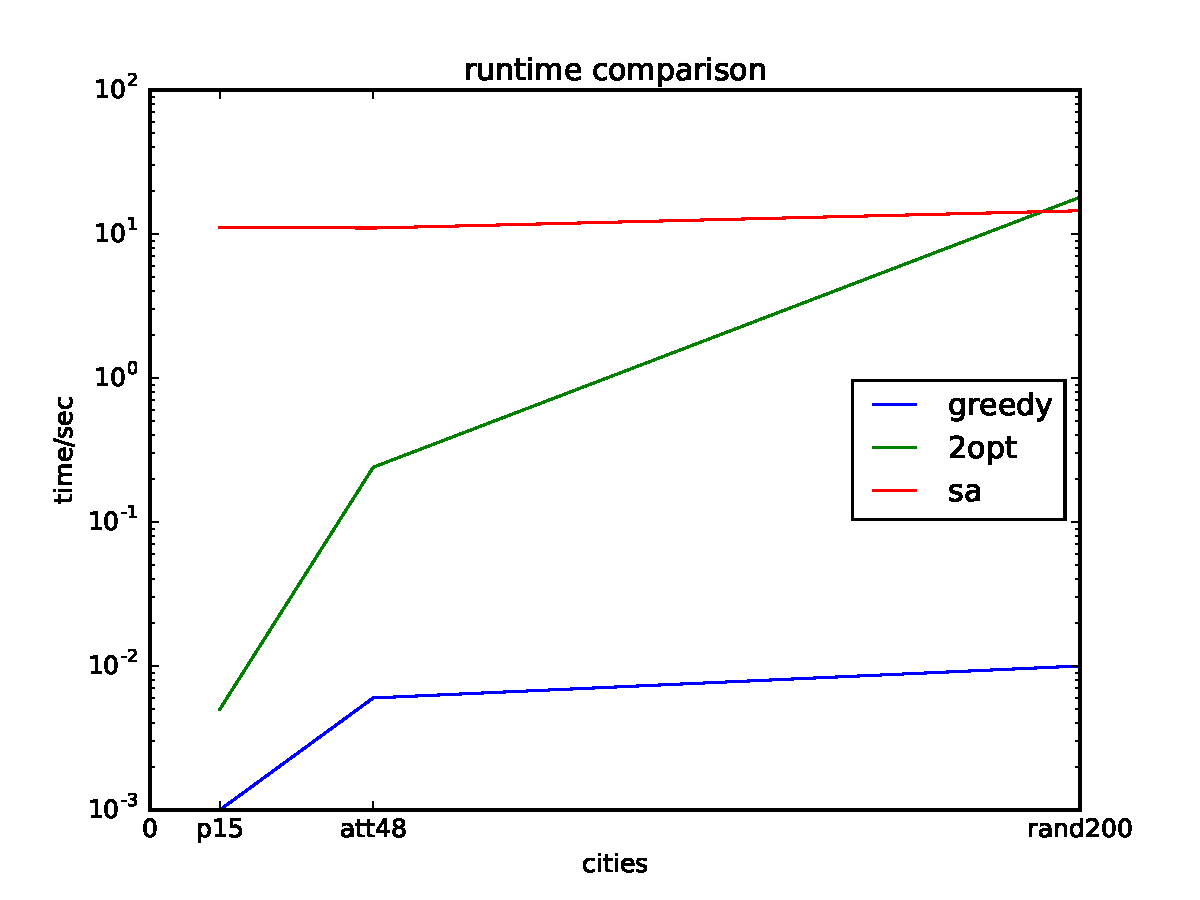
\includegraphics[width=.7\linewidth]{time}
	\caption{时间消耗分析}
	\label{fig:time}
\end{figure}



\section{实验总结}
通过上面分析可以看出,\huo 无法被完美解决,但是在数据集较大的情况下,还是能给出不错的亚最优的结果。通过本次实验,我巩固了人工智能方面的知识,增强了对人工智能的好奇心。

最终还要感谢相明老师的耐心指导。

{\small
	\bibliographystyle{ieee}
	\bibliography{he16tsp}
}
\end{CJK}
\end{document}
